\documentclass[12pt,aspectratio=169]{beamer}
\usepackage{tikz}
\usetheme{Madrid}
\setbeamertemplate{navigation symbols}{}
\title{Iterative refinement: experiments and bounds}
\subtitle{Generated interaction study}
\author{Research group}
\date{}
\year=2026\month=11\day=5
\newcommand{\fuzzlayerA}[1]{\textbf{#1}}
\newcommand{\fuzzterm}[1]{\fuzzlayerA{#1}}
\newcommand{\fuzzpair}[2]{\fuzzterm{#1}: #2}
\newcommand{\fuzzunit}{steps}
\let\fuzzoriginalunit\fuzzunit
\newcommand{\fuzzcoefficient}{4}
\newcommand{\fuzzscale}[2][\fuzzcoefficient]{#1\,#2}
\definecolor{fuzzpaint}{RGB}{255,0,255}
\definecolor{fuzzsecond}{RGB}{18,137,67}
\tikzset{fuzzvertex/.style={draw,rounded corners=1pt,fill=blue!10,inner sep=1pt,minimum width=.35cm,minimum height=.25cm}}
\begin{document}\begin{frame}[t]{Picture tail}\relax {\small\color{blue}\raggedright \begin{alertblock}{Message passing}
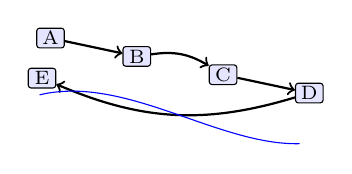
\begin{tikzpicture}[font=\scriptsize]
\begin{scope}[scale=0.8,rotate=-12]


\node[fuzzvertex] (g6n0) at (0.000,0) {A};
\node[fuzzvertex] (g6n1) at (1.400,0) {B};
\node[fuzzvertex] (g6n2) at (2.800,0) {C};
\node[fuzzvertex] (g6n3) at (4.200,0) {D};
\node[fuzzvertex] (g6n4) at (0.000,-0.65) {E};
\begin{scope}[xshift=.5pt,yshift=-.5pt]
\draw<2->[->,thick] (g6n0) -- (g6n1);
\draw<2->[->,thick] (g6n1) to[bend left=20] (g6n2);
\draw<2->[->,thick] (g6n2) -- (g6n3);
\draw<2->[->,thick] (g6n3) to[bend left=20] (g6n4);
\draw[blue] (0,-.9) .. controls (1.260,-.3) and (2.940,-1.1) .. (4.200,-.8);
\end{scope}
\end{scope}
\end{tikzpicture}
\end{alertblock}
After.\par}\end{frame}\end{document}